%\part{Linux系统管理}
%\section{用户管理}

%

%
%\subsection{增加用户}
%
%
%\begin{frame}{增加用户帐号}
%\begin{itemize}
%	\item 最通常做法是执行useradd指令
%	
%	\begin{itemize}
%		\item useradd \emph{{[}options{]} username}
%	\end{itemize}
%	\item 运行useradd等价于
%	
%		\begin{itemize}
%			\item 编辑/etc/\{passwd,shadow,group,gshadow\}
%			\item 创建和填充用户的主目录(/etc/skel)
%			\item 设置许可和所有权
%		\end{itemize}
%	\item 使用passwd设置密码
%	\item 用newusers批处理增加帐号
%\end{itemize}
%
%\end{frame} 
%
%
%\begin{frame}{用户私有组}
%\begin{itemize}
%\item 用户帐号创建时,一个同名的私有组也同时创建
%
%\begin{itemize}
%\item 用户默认属于这个私有组
%\item 用户的新文件都属于这个组
%\end{itemize}
%\item 好处:防止新文件属于公共组,私密考虑
%\item 缺点:有鼓励设置文件为全局可读的倾向
%\end{itemize}
%
%\end{frame} 
%\begin{frame}{修改/删除用户帐号}
%\begin{itemize}
%\item 改变/etc/passwd文件的一些项值,你可以
%
%\begin{itemize}
%\item 手工编辑该文件
%\item 使用 usermod \emph{{[}options{]} username}
%\end{itemize}
%\item 删除一个帐号可以用以下方法之一
%
%\begin{itemize}
%\item 手工删除/etc/\{passwd,shadow,group,gshadow\},/var/spool/mail等文件的用户信息
%\item 使用 userdel \emph{{[} -r {]} username}
%\end{itemize}
%\end{itemize}
%
%\end{frame} 
%\begin{frame}{管理用户组}
%\begin{itemize}
%\item 本质上是在/etc/\{group,gshadow\}文件中增加或者修改条目信息
%
%\begin{itemize}
%\item groupadd
%\item groupmod
%\item groupdel
%\end{itemize}
%\end{itemize}
%
%\end{frame} 
%\begin{frame}{密码和时效性策略}
%\begin{itemize}
%\item 缺省情况下,密码不过期
%\item 强制密码过期是安全策略的一部分
%\item 通过/etc/login.defs修改缺省的过期设置
%\item 通过chage命令可以修改已有账户的密码期限
%
%\begin{itemize}
%\item chage \emph{{[}options{]} username}
%\end{itemize}
%\end{itemize}
%
%\end{frame} 
%\begin{frame}{切换账户}
%\begin{itemize}
%\item 可以在不注销的情况下,随时切换到其他已有账户环境下
%\item 语法
%
%\begin{itemize}
%\item su {[} - {]} {[} user {]}
%\item su {[} - {]} {[} user {]} -c \emph{command}
%\end{itemize}
%\item 允许当前账户临时变成另外一个账户,缺省是变成root
%\item -,表示创建新的shell环境
%\end{itemize}
%\end{frame} 
%\subsection{特殊许可}
%
%
%
%\begin{frame}{SUID/SGID可执行程序}
%\begin{itemize}
%\item 普通用户如何修改其密码?
%\item 某一个账户运行的进程限制在当前账户的权限上下文环境里
%\item SUID/SGID位的设置,可以使得该程序被执行时,获得的不是程序发起账户而是文件所有者的上下文环境
%\item /bin/mount,/usr/bin/passwd,etc
%\end{itemize}
%
%\end{frame} 
%\begin{frame}{SGID目录}
%
%
%\begin{itemize}
%\item 用来创建协同工作目录
%\item 通常情况下,在目录下创建的文件属于该账户的缺省组
%\item 但是在有SGID位设置的目录下,创建的文件却和该目录属于同一个组
%\item \$ ls -ld a\\
%drwxrw\alert{s}rwx 2 wgzhao wgzhao 4096 2009-10-16 11:27 \\
%\$ ls -l a
%
%
%total 0
%
%
%-rw-r--r-- 1 oracle wgzhao 0 2009-10-16 11:27 oracle
%
%
%-rw-r--r-- 1 wgzhao wgzhao 0 2009-10-16 11:27 wgzhao
%
%\end{itemize}
%
%\end{frame} 
%\begin{frame}{粘滞位 stickly bit}
%
%
%\begin{itemize}
%\item 通常情况下,如果账户对某一个目录有写的许可,就意味着他能删除该目录下的任何文件,而不用考虑文件本身的许可
%\item 但是设置粘滞位后,账户就只能删除属于自己的文件
%\item ls -ld /tmp\\
%drwxrwxrw\alert{t} 17 root root 24576 2009-10-16 11:36 /tmp
%\end{itemize}
%\end{frame} 
%\subsection{实验}
%
%
%
%\begin{frame}{实验I:创建组和用户}
%
%
%\begin{description}
%\item [{场景:}] 你需要为公司不同的部门设置不同的组。同时,你也需要为每一个部门的职员设置帐号
%\item [{要求:}] 系统用户eva和basten在sales组;katherine和lily在hr组;john和crix在web组;manager在sales,hr和web组
%\end{description}
%提示:
%\begin{enumerate}
%\item 确保所有新创建的用户可以创建组可写文件
%\item 设定GID
%\item 私有组,辅助组
%\end{enumerate}
%
%\end{frame} 
%\begin{frame}{实验II:设置共享目录}
%
%
%\begin{description}
%\item [{场景:}] 接上一个场景,你为每一个部门创建的组,同时也需要一个共享目录。\\
%它允许每一个部门内职员共享文件,但是防止其他部门职员修改,甚至看到文件
%\item [{要求:}] 每一个部门的共享目录仅允许部门内职员帐号进入或者在目录内创建,查看和修改文件
%\end{description}
%提示:
%\begin{enumerate}
%\item 创建/depts目录以及sales,hr和web子目录
%\item 设置每一个目录的组所有者
%\item 设置相关权限
%\end{enumerate}
%\end{frame} 


\section{文件系统管理}
\begin{frame}{系统管理}
	\tableofcontents[currentsection]
\end{frame} 

%\begin{frame}{文件系统}
%目标
%\begin{itemize}
%\item 理解文件系统层次结构
%\item 管理交换分区
%\item 增加新的设备于分区
%\item 挂载NFS文件系统
%\end{itemize}
%
%\end{frame} 

%\begin{frame}{概览:增加新文件系统}
%
%要添加一个新的文件系统到系统中,遵循下列步骤:
%\begin{enumerate}
%\item 识别设备
%\item 对设备进行分区(如有必要)
%\item 创建文件系统
%\item 标识文件系统,便于管理(可选)
%\item 在/etc/fstab增加新条目(可选)
%\item 挂载新的文件系统
%\end{enumerate}
%\end{frame} 

\subsection{设备与分区}

\begin{frame}{磁盘分区}
\begin{itemize}
\item 内核支持的最大分区数:

\begin{itemize}
\item IDE设备,63个
\item SCSI设备,15个
\end{itemize}
\item 为什么要分区?

\begin{itemize}
\item 容量
\item 性能
\item 配额
\item 恢复
\end{itemize}
\end{itemize}

\end{frame} 
\begin{frame}{管理分区}
\begin{itemize}
\item 使用下列程序来创建和管理分区:

\begin{itemize}
\item fdisk
\item sfdisk
\item GNU parted 高级分区处理
\end{itemize}
\item partprobe 
\end{itemize}

\end{frame} 
\begin{frame}{fdisk}
\begin{itemize}
\item 查看和管理分区表
\item 从命令行列出分区表

\begin{itemize}
\item fdisk -l
\end{itemize}
\item 交互模式管理分区表

\begin{itemize}
\item fdisk \emph{/dev/sda}
\end{itemize}
\item partprobe
\item cat /proc/partitions
\end{itemize}
\end{frame} 

\subsection{文件系统创建与调整}

\begin{frame}{创建文件系统}
\begin{itemize}
\item mkfs
\item mkfs.ext2,mkfs.ext3,mkfs.ext4,mkfs.msdos
\item 特殊文件系统工具可以直接调用

\begin{itemize}
\item mke2fs \emph{{[} options {]} device}
\end{itemize}
\end{itemize}

\end{frame} 
\begin{frame}{文件系统标签(label)}
\begin{itemize}
\item 引用设备的另一方法
\item 设备独立性,不受特定设备名约束

\begin{itemize}
\item e2label \emph{special\_dev\_file {[} fslabel {]}}
\item mount \emph{{[} options {]}} LABEL=\emph{fslabel mount\_point}
\end{itemize}
\item blkid 可以查看所有设备的标签,文件系统类型以及UUID号 
\begin{exampleblock}{}
\# blkid -o value -s UUID /dev/sda2 \\
f252a71d-cf7d-4166-8315-cda1e217a08c
\end{exampleblock}
\end{itemize}
\end{frame} 


\begin{frame}{tune2fs}
\begin{itemize}
\item tune2fs 用来调整文件系统参数

\begin{itemize}
\item 保留块,缺省是5\%
\item 缺省挂载选项,缺省是defaults
\item fsck的频率,缺省是挂载次数30次,时长180天
\end{itemize}
\item dumpe2fs 查看当前设置
\end{itemize}
\end{frame} 

\subsection{挂载}

\begin{frame}{挂载点和/etc/fstab}
\begin{itemize}
\item 系统层次结构的配置文件
\item 被mount,fsck及其他工具使用
\item 系统重启后还能维持层次结构
\item /etc/fstab中的设备域可以用标签(label)替代,推荐这样做!
\item mount -a 能挂载所有在/etc/fstab里设定的文件系统,有noauto标志除外
\end{itemize}

\end{frame} 
\begin{frame}{用mount挂载文件系统}
\begin{itemize}
\item mount \emph{{[} options {]}} \emph{device mount\_point}

\begin{itemize}
\item -t 指定文件系统类型,一般不需要
\item -o 挂载选项,缺省挂载选项为
\item rw,suid,dev,exec,acl,async
\end{itemize}
\end{itemize}

\end{frame} 
\begin{frame}{卸载文件系统}
\begin{itemize}
\item umount \emph{{[} options {]} device | mount\_point}
\item 不能卸载仍在被使用的文件系统

\begin{itemize}
\item 使用fuser检查或杀死进程
\end{itemize}
\item 使用remount选项可以在自动改变挂载选项

\begin{itemize}
\item mount -o remount,ro /dev/sda1 /data
\end{itemize}
\end{itemize}
\end{frame} 

\subsection{特定文件系统}

\begin{frame}{交换空间 swap}
\begin{itemize}
\item 交换空间是对物理内存的有效补充
\item 基本设置步骤:

\begin{itemize}
\item 创建一个交换分区或者文件
\item 使用mkswap写入分区特征信息
\item 在/etc/fstab增加正确的条目
\item 使用swapon -a激活交换空间
\end{itemize}
\end{itemize}

\end{frame} 
\begin{frame}{挂载NFS文件系统}
\begin{itemize}
\item 把远程的目录当作本地文件系统来挂载使用
\item /etc/fstab支持NFS挂载配置
\item 通过/etc/init.d/netfs可以自动挂载NFS
\item 手工挂载方式

\begin{itemize}
\item mkdir /mnt/srv1-nfs
\item mount -t nfs \emph{srv1:/data/shared /mnt/srv1-nfs}
\end{itemize}
\end{itemize}
\end{frame} 

%\subsection{实验}
%
%
%
%\begin{frame}{实验 I: 创建新的文件系统}
%\begin{description}
%\item [{场景:}] 新的应用程序需要安装到/opt目录。基于恢复的原因,/opt需要成为单独的分区,新的/opt分区重启后依然有效
%\item [{要求:}] 系统提供独立分区挂载到/opt
%\end{description}
%提示:
%\begin{enumerate}
%\item 创建新的分区(fdisk/parted)
%\item 创建文件系统(mkfs,mke2fs)
%\item 修改/etc/fstab
%\end{enumerate}
%
%\end{frame} 
%\begin{frame}{实验II:创建新的交换空间}
%\begin{description}
%\item [{场景:}] 系统目前的交换分区已经不够用,需要增加交换分区,但是不能影响现有的其他分区。所有的交换分区都应该在系统重启后仍然激活
%\item [{要求:}] 给系统增加一个交换分区
%\end{description}
%提示:
%\begin{enumerate}
%\item 创建新分区
%\item 创建交换系统
%\item 激活测试
%\item 持久化
%\end{enumerate}
%
%\end{frame} 
%\begin{frame}{实验III:挂载实践}
%\begin{description}
%\item [{要求:}] 使用合适的挂载参数来完成下面的需求
%
%\begin{itemize}
%\item 禁止可执行访问
%\item 挂载一个文件系统镜像
%\item 挂载非Linux文件系统
%\item 禁止访问时间更新
%\item 设置一个挂载别名
%\end{itemize}
%\end{description}
%\end{frame} 


\section{包管理}

\begin{frame}{包管理}

%目标:
%\begin{itemize}
%\item 安装和删除RPM包
%\item 查询包和校验状态
%\item 使用yum管理包
%\item 了解yum和rpm的关系
%\item 利用yum来在线更新包
%\item 制作RPM包
%\end{itemize}
\tableofcontents[currentsection]
\end{frame} 

\subsection{RPM包管理}

\begin{frame}{RPM包管理}
\begin{itemize}
\item RPM(\alert{R}edhat \alert{P}ackages \alert{M}anager) 组件:

\begin{itemize}
\item 本地数据库
\item rpm和相关可执行程序
\item rpm前端程序如yum
\item 包文件
\end{itemize}
\item 基本功能:

\begin{itemize}
\item 安装/删除
\item 查询
\item 校验
\end{itemize}
\end{itemize}
\end{frame} 

\subsection{安装和删除软件}



\begin{frame}{安装和删除软件}
\begin{itemize}
\item 基本rpm指令参数:

\begin{itemize}
\item 安装 rpm -i,--install
\item 升级 rpm -U, --upgrade
\item 刷新 rpm -F,--freshen
\item 
\item 删除 rpm -e,--erase
\end{itemize}
\item 输出选项: -v,-h
\item URL支持: ftp://,http://
\end{itemize}
\end{frame} 

\subsection{更新内核RPM包}


\begin{frame}{更新内核RPM包}
\begin{itemize}
\item 真的需要更新内核?
\item \alert{不要使用rpm -U,rpm -F方式更新内核}

\begin{itemize}
\item rpm -ivh kernel-version.arch.rpm
\item 启动新内核,测试
\item 如果新内核有问题,回退到旧内核
\item 如果没有问题,删除旧内核 rpm -e kernel-oldversion
\end{itemize}
\end{itemize}
\end{frame} 

\subsection{rpm指令}



\begin{frame}{rpm查询}
\begin{itemize}
\item 语法:

\begin{itemize}
\item rpm -q what\_packages what\_information
\end{itemize}
\item 查询已安装选项

\begin{itemize}
\item rpm -qa 列出已经安装的包
\item rpm -qf filename 查询filename属于那个包
\item rpm -qi pkg 显示包pkg的一般信息
\item rpm -ql pkg 列出包pkg安装的文件
\end{itemize}
\item 查询未安装包选项

\begin{itemize}
\item rpm -qip pkg.i386.rpm 显示一般信息
\item rpm -qlp pkg.i36.rpm 列出包含的文件
\end{itemize}
\end{itemize}

\end{frame} 
\begin{frame}{rpm校验}
\begin{itemize}
\item 已安装的rpm包校验

\begin{itemize}
\item rpm -V pkg\_name
\item rpm -Vp pkg\_name.i386.rpm
\item rpm -Va
\end{itemize}
\item 包安装前校验签名

\begin{itemize}
\item rpm --import RPM-GPG-KEY
\item rpm -K pkg\_name.i386.rpm
\end{itemize}
\end{itemize}

\end{frame} 
\begin{frame}{关于yum}
\begin{itemize}
\item rpm的前端程序

\begin{itemize}
\item 旨在解决包依赖关系
\item 能跨软件源找到包
\end{itemize}
\end{itemize}

\end{frame} 
\begin{frame}{使用yum}
\begin{itemize}
\item 安装/删除/更新

\begin{itemize}
\item yum install \emph{package} \ldots{}
\item yum remove \emph{package} \ldots{}
\item yum update {[} \emph{package} \ldots{} {]}
\end{itemize}
\item 搜索包/文件
\item 搜索包

\begin{itemize}
\item yum search \emph{searchterm}
\item yum list (all|available|extras|installed|recent|updates)
\item yum info \emph{packagename}
\end{itemize}
\item 搜索文件

\begin{itemize}
\item yum whatprovides \emph{filename}
\end{itemize}
\end{itemize}
\end{frame} 

%\begin{frame}{配置其他软件库(Repository)}
%\begin{itemize}
%\item 给库创建一个文件,保存在/etc/yum.repos.d/目录,后缀为.repo
%\item 必要的一些信息
%
%\begin{itemize}
%\item {[}\emph{repo-name}{]}
%\item name= \emph{A nice description}
%\item baseurl = \emph{http://yourserver.com/path/to/repo}
%\item enabled=1
%\item gpgcheck=1
%\end{itemize}
%\item 仓库信息缓存到本地,使用下面的命令清除:
%
%\begin{itemize}
%\item yum clean dbcache | all
%\end{itemize}
%\end{itemize}
%
%\end{frame} 
%\begin{frame}{创建自己的软件库}
%\begin{itemize}
%\item 创建目录,将软件包存放到此
%\item 使得该目录能够通过http/ftp 访问
%\item 安装 createrepo RPM包
%\item 运行 createrepo -v \emph{/package/directory}
%\item 将创建 repodata 子目录以及其他必要的支持文件
%\end{itemize}
%\end{frame} 

\subsection{制作RPM包}

\begin{frame}{制作RPM包}
在目前的Linux环境下,要安装新软件,通常有两种方式:一是使用源码安装;二是使用rpm软件包。使用源码安装可以让用户了解编译过程,及定制一些模块,和修改编译参数,但其工作量通常都很大,而且要求用户有足够的计算机知识。而rpm软件包方式则相对来说比较简单,也易于管理和升级。所以,当前Linux发行版的前十中,有八个都是使用基于二进制软件包方式的(deb和rpm格式可以互转)。
\end{frame}

\begin{frame}{目录准备}
/usr/src/asianux/ \\
|-- BUILD   ---编译时的工作目录,包括解压和make都会放到这里 \\
|-- RPMS   ---根据硬件平台的不同,存放最后生成的RPM软件包 \\
|-- SOURCES ---存放源码包的地方,一般带压缩的tar包 \\
|-- SPECS ---存放编译RPM时的.spec脚本 \\
|-- SRPMS ---存放编译好的.src.rpm软件包 \\
\end{frame}

\begin{frame}[plain]{rpm制作流程}
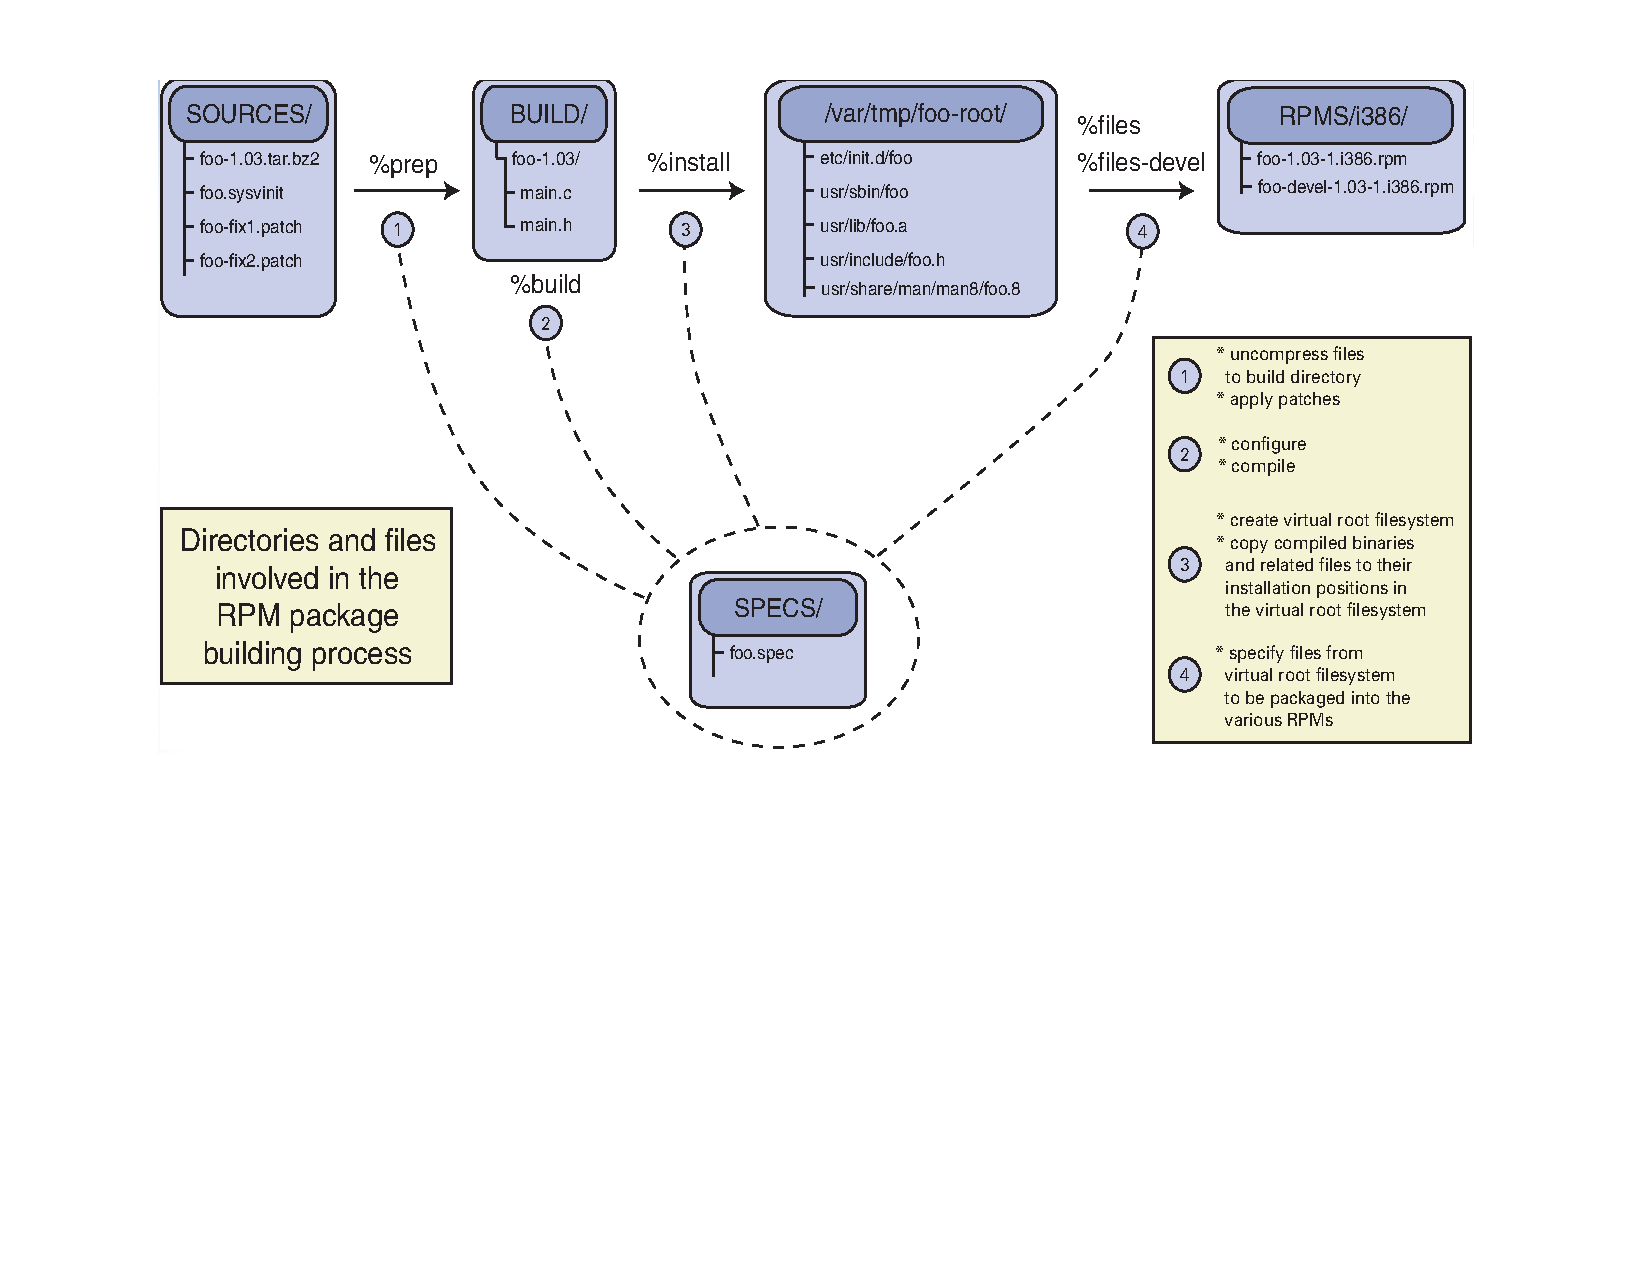
\includegraphics[scale=.5]{rpm-build-flowcharts} \footnote{http://www.gurulabs.com/GURULABS-RPM-LAB/GURULABS-RPM-GUIDE-v1.0.PDF}
\end{frame}

\begin{frame}[fragile]{自定义目录}
\begin{verbatim}
echo "%_topdir $HOME/rpm" >> $HOME/.rpmmacros
mkdir $HOME/rpm
mkdir $HOME/rpm/SOURCES
mkdir $HOME/rpm/SPECS
mkdir $HOME/rpm/BUILD
mkdir $HOME/rpm/SRPMS
mkdir $HOME/rpm/RPMS
mkdir $HOME/rpm/RPMS/i386
echo '%debug_package %{nil}' >> ~/.rpmmacros  
		#does not create debuginfo rpm package
\end{verbatim}
\end{frame}

\begin{frame}{从rpm源代码创建rpm包}
\begin{enumerate}
\item  下载需要的rpm源代码包,后缀一般是src.rpm
\item 执行下面的指令来直接编译: \\
rpmbuild -{}-rebuild foo-<version>.src.rpm
\item 如果编译正常,生成的rpm包放在 \\
/usr/src/asianux/RPMS/目录下
\end{enumerate}
\end{frame}


\begin{frame}{rpmbuild 常用参数}
\begin{description}
\item[-{}-rebuild] 从源代码包编译二进制包
\item[-ba] 从spec文件编译源代码包和二进制包
\item[-bb] 从spec文件仅编译二进制包
\item[-bs] 从spec文件仅编译源代码包
\item[-ta] 从tar包编译源代码和二进制包
\item[-tb] 从tar包仅编译二进制包
\item[-ts] 从tar包仅编译源代码包
\end{description}
注意: \\
这里说的源代码包是指后缀为.src.rpm的包 \\
spec文件说的是后缀为.spec文件 \\
tar包说的是以.tar.gz/.tar.bz2等格式的源代码 \\
二进制包指的是后缀为.rpm的包
\end{frame}

\begin{frame}[fragile,allowframebreaks]{spec文件说明:关键字}
spec文件包括很多关键字,主要有
\begin{description}
\item[Name] 软件包的名字,后面可以使用\%\{name\} 的方式引用
\item[Summary] 软件包的内容摘要
\item[Version] 软件的实际版本号,例如 2.1.4,后面可以用\%\{version\}引用
\item[Release] 发布序列号,比如12,标明第几次打包,后面可用\%\{release\}引用
\item[Group] 软件分组,建议使用标准分组
\item[License] 软件授权方式,GPL,LGPL,BSD,MPL, MIT,$\cdots$
\item[Source] 源代码包,可以带多个用Source1,Source2等源,后面可以用\%\{source1\},\%\{source2\}引用
\item[BuildRoot] 这个是安装或编译时使用的“虚拟目录”,考虑到多用户的环境,一般定义为:\\
\%\{\_tmppath\}/\%\{name\}-\%\{version\}-\%\{release\}-root \\
或 \\
\%\{\_tmppath\}/\%\{name\}-\%\{version\}-\%\{release\}-buildroot-\%(\%\{\_\_id\_u\} -n\} \\
该参数非常重要,因为在生成rpm的过程中,执行make install时就会把软件安装到上述的路径中,在打包的时候,同样依赖“虚拟目录”为“根目录”进行操作。
后面可使用\$RPM\_BUILD\_ROOT 方式引用
\item[URL] 软件的主页
\item[Vendor]发行商或打包组织的信息,例如BaseSoft Co,.Ltd.
\item[Patch] 补丁代码,可以使用Patch1,Patch2等标识多个补丁,后面使用\%patch0 或\%\{patch0\} 引用
\item[Prefix: \%\{\_prefix\}] 这个主要是为了解决今后安装rpm包时,并不一定把软件安装到rpm中打包的目录的情况。这样,必须在这里定义该标识,并在编写\%install脚本的时候引用,才能实现rpm安装时重新指定位置的功能
\item[Prefix: \%\{\_sysconfdir\}] 这个原因和上面的一样,但由于\%\{\_prefix\}指/usr,而对于其他的文件,例如/etc下的配置文件,则需要用\%\{\_sysconfdir\}标识
\item[Build Arch] 指编译的目标处理器架构,noarch标识不指定,但通常都是以/usr/lib/rpm/marcros中的内容为默认值

\item[Requires] 该rpm包所依赖的软件包名称,可以用>=或<=表示大于或小于某一特定版本,例如:\\
libpng-devel >= 1.0.20 zlib \\ 
“>=”号两边需用空格隔开,而不同软件名称也用空格分开
还有例如PreReq、Requires(pre)、Requires(post)、Requires(preun)、Requires(postun)、BuildRequires等都是针对不同阶段的依赖指定 

\item[Provides] 指明本软件一些特定的功能,以便其他rpm识别

\item[Packager] 打包者的信息

\item[\%description] 软件的详细说明
\end{description}

\end{frame}

\begin{frame}[allowframebreaks]{spec文件说明:脚本主体 }
spec脚本的主体中也包括了很多关键字和描述
\begin{description}
\item[\%prep] 预处理脚本
\item[\%setup -n \%\{name\}-\%\{version\}]把源代码解压并放好 \\
通常是从/usr/src/asianux/SOURCES里的包解压到/usr/src/asianux/BUILD/\%\{name\}-\%\{version\}中。
一般用\%setup -c就可以了,但有两种情况:一就是同时编译多个源码包,二就是源码的tar包的名称与解压出来的目录不一致,此时,就需要使用-n参数指定一下了。
\item[\%patch] 打补丁 \\
通常补丁都会一起在源码tar.gz包中,或放到SOURCES目录下。一般参数为:
\%patch -p1 使用前面定义的Patch补丁进行,-p1是忽略patch的第一层目录
\%Patch2 -p1 -b xxx.patch 打上指定的补丁,-b是指生成备份文件

\item[\%configure] 这个不是关键字,而是rpm定义的标准宏命令。意思是执行源代码的configure配置 \\
在/usr/src/asianux/BUILD/\%\{name\}-\%\{version\}目录中进行 ,使用标准写法,会引用/usr/lib/rpm/marcros中定义的参数。

\item[\%build] 开始构建包 \\
在/usr/src/asianux/BUILD/\%\{name\}-\%\{version\}目录中进行make的工作,常见写法: \\
make \%\{?\_smp\_mflags\} OPTIMIZE="\%\{optflags\}" \\
都是一些优化参数,定义在/usr/lib/rpm/marcros中

\item[\%install] 开始把软件安装到虚拟的根目录中
在/usr/src/asianux/BUILD/\%\{name\}-\%\{version\}目录中进行make install的操作。这个很重要,因为如果这里的路径不对的话,则下面\%file中寻找文件的时候就会失败。
\item[\%clean] 清理临时文件
%通常内容为 
%\begin{verbatim}
%[ "$RPM_BUILD_ROOT" != "/" ] && rm -rf "$RPM_BUILD_ROOT"
%rm -rf $RPM_BUILD_DIR/%{name}-%{version}
%\end{verbatim}
%\alert{\$RPM\_BUILD\_ROOT 是指开头定义的BuildRoot,\\ \$RPM\_BUILD\_DIR 通常就是指/usr/src/asianux/BUILD,其中,前面的才是 \%file 需要的。}

\item[\%pre] rpm安装前执行的脚本
\item[\%post] rpm安装后执行的脚本

\item[\%preun] rpm卸载前执行的脚本

\item[\%postun] rpm卸载后执行的脚本

\item[\%files] 定义哪些文件或目录会放入rpm中 \\
\alert{这里会在虚拟根目录下进行,千万不要写绝对路径,而应用宏或变量表示相对路径}
\item[\%defattr(-,root,root)] 指定包装文件的属性,分别是(mode,owner,group),-表示默认值,对文本文件是0644,可执行文件是0755

\item[\%exclude] 列出不想打包到rpm中的文件 \\
\alert{如果指定的文件不存在,也会出错的} 
\item[\%changelog] 变更日志
\end{description}
\end{frame}


\begin{frame}[allowframebreaks]{foobar.spec 简析}
\lstinputlisting{scripts/foobar.spec}
\end{frame}

\begin{frame}{参考资料}
\begin{itemize}
\item \href{http://fedoranews.org/alex/tutorial/rpm/}{RPM Tutorial}
\item \href{http://docs.fedoraproject.org/en-US/Fedora_Draft_Documentation/0.1/html/RPM_Guide/index.html}{Fedora RPM Guide}
\item \href{http://www.gurulabs.com/GURULABS-RPM-LAB/GURULABS-RPM-GUIDE-v1.0.PDF}{Create RPMs}
\item \href{http://docs.fedoraproject.org/en-US/Fedora_Draft_Documentation/0.1/html/RPM_Guide/ch-rpm-programming-python.html} {Programming RPM with Python} 
\end{itemize}
\end{frame}

%\subsection{软件包实验}
%
%
%
%\begin{frame}{实验I:使用RPM}
%\begin{itemize}
%\item 插入第一张光盘,进入到/media/cdrom/Asianux/RPMS目录,完成下面的问题
%
%\begin{enumerate}
%\item 使用rpm -i util-linux来安装util-linux软件包,应该会失败,纠正这个问题
%\item initscripts 包有哪些文件?
%\item pam软件包自安装后是否有过改动,如果有,改动了哪些文件?
%\item /bin/grep 文件是哪个包提供的?
%\item /etc/hosts是那个软件包提供的,为什么?
%\end{enumerate}
%\end{itemize}
%
%\end{frame} 
%\begin{frame}{实验II:连接到软件库}
%\begin{description}
%\item [{场景:}] firefox浏览器没有默认不提供flash的支持,请创建flash软件的仓库,确保能连接到仓库
%\item [{要求:}] 配置包含adobe软件的仓库
%\end{description}
%
%\end{frame} 
%\begin{frame}{实验III:用yum安装新软件}
%\begin{description}
%\item [{要求:}] 使用yum安装flash插件
%\end{description}
%
%\end{frame} 
%\begin{frame}{实验IV:用yum更新软件}
%\begin{description}
%\item [{要求:}] 针对你想要更新的软件包,在网络上找到对应的仓库,并更新
%\end{description}
%\end{frame} 
%\section{网络配置}
%
%
%
%\begin{frame}{网络配置}
%
%目标
%\begin{itemize}
%\item 配置IP接口
%\item 设置路由
%\item 理解名字解析
%\end{itemize}
%\end{frame} 
%
%\subsection{概述}
%
%
%
%\begin{frame}{网络接口}
%\begin{itemize}
%\item 网络配置脚本需要涉及到设备的逻辑名
%
%\begin{itemize}
%\item 以太网:eth0,eth1 \ldots{}
%\item 拨号:ppp0,ppp1 \ldots{}
%\item 回路:lo
%\end{itemize}
%\item 显示网络接口
%
%\begin{itemize}
%\item ifconfig -a
%\item ip link {[} show {]}
%\end{itemize}
%\end{itemize}
%
%\end{frame} 
%\begin{frame}{驱动选择}
%\begin{itemize}
%\item 所有的网卡驱动都编译成内核模块
%\item /etc/modprobe.conf 将网卡逻辑名映射到特性的内核模块上
%
%\begin{itemize}
%\item alias eth0 bnx2
%\end{itemize}
%\item 通过/etc/sysconfig/network-scripts/ifcfg-eth0的配置也能选定特定网卡
%
%\begin{itemize}
%\item HWADDR=00:12:34:00:00:00
%\end{itemize}
%\end{itemize}
%
%\end{frame} 
%\begin{frame}{速率和双工设置}
%\begin{itemize}
%\item 缺省情况下,速率和双工配置是自动协商的
%\item 速率,双工与设备或者网络不匹配会导致通讯的断断续续
%\item 可以手工设定参数
%
%\begin{itemize}
%\item ethtool
%\item ifcfg-ethX里设置ETHTOOL\_OPTS参数
%\item 如果内核模块支持,在/etc/modprobe.conf里加入options或install 选项
%\end{itemize}
%\end{itemize}
%\end{frame} 
%
%\subsection{IPv4配置}
%
%
%
%\begin{frame}{IPv4地址}
%
%查看配置
%\begin{itemize}
%\item ifconfig
%\item ip addr {[} show {]}
%\end{itemize}
%
%\end{frame} 
%\begin{frame}{动态IPv4配置}
%\begin{itemize}
%\item 配置文件
%
%\begin{itemize}
%\item /etc/sysconfig/network-scripts/ifcfg-\emph{ethX}
%\item BOOTPROTO=dhcp 表示动态配置IPv4地址
%\end{itemize}
%\end{itemize}
%
%\begin{itemize}
%\item 使用ifdown \emph{device};ifup \emph{device} 应用新的配置
%\end{itemize}
%
%\end{frame} 
%\begin{frame}{静态IPv4配置}
%\begin{itemize}
%\item 配置文件
%
%\begin{itemize}
%\item /etc/sysconfig/network-scripts/ifcfg-\emph{ethX}
%\end{itemize}
%\item 配置的必要内容:
%
%\begin{itemize}
%\item DEVICE=\emph{ethX}
%\item BOOTPROTO=none
%\item IPADDR=\emph{192.168.6.4}
%\item NETMASK=\emph{255.255.255.0}
%\end{itemize}
%\end{itemize}
%
%\end{frame} 
%\begin{frame}{设备别名}
%\begin{itemize}
%\item 对于虚拟主机,高可用软件而言特别有用
%\item 可以在一块网卡上绑定多个IP地址
%
%\begin{itemize}
%\item eth0:0
%\item eth0:1
%\item eth0:2
%\end{itemize}
%\item 每一个设备别名都可以创建独立的配置文件
%
%\begin{itemize}
%\item ifcfg-\emph{ethX:xxx}
%\item 只能使用静态网络设置
%\end{itemize}
%\end{itemize}
%\end{frame} 
%
%\subsection{路由配置}
%
%
%
%\begin{frame}{路由表}
%\begin{itemize}
%\item 定义到所有系统的网络路径
%\item 查看路由表方法
%
%\begin{itemize}
%\item route {[} -n {]}
%\item netstat -r {[} -n {]}
%\item ip route {[} show {]}
%\end{itemize}
%\end{itemize}
%
%\end{frame} 
%\begin{frame}{缺省网关}
%\begin{itemize}
%\item 没有路由匹配时而使用的路由称为缺省网关
%\item 可以通过DHCP获得
%\item 也可以静态设置
%
%\begin{itemize}
%\item /etc/sysconfig/network 里增加
%\item GATEWAY=192.168.6.1
%\item 或者,在每一个网卡配置文件里加入\\
%/etc/sysconfig/network-scripts/ifcfg-\emph{ethX}
%\end{itemize}
%\end{itemize}
%
%\end{frame} 
%\begin{frame}{配置路由}
%\begin{itemize}
%\item 静态配置方法:
%
%\begin{itemize}
%\item 每一个网卡有一个路由配置文件\\
%/etc/sysconfig/network-scripts/route-\emph{ethX}
%\item 使用 ip route add / route add 语法
%\end{itemize}
%\item 通过守护进程学习动态路由
%
%\begin{itemize}
%\item quagga
%\item 支持RIP,OSPF,BGP等各种协议
%\end{itemize}
%\end{itemize}
%
%\end{frame} 
%\begin{frame}{校验IP连通性}
%\begin{itemize}
%\item ping
%
%\begin{itemize}
%\item 网络包丢失和延迟测量工具
%\end{itemize}
%\item traceroute
%
%\begin{itemize}
%\item 显示到某一个目的地的网络路径
%\end{itemize}
%\item mtr
%\end{itemize}
%
%\end{frame} 
%\begin{frame}{定义本地主机名}
%\begin{itemize}
%\item hostname 查看/设置本地主机名
%\item 在/etc/sysconfig/network定义主机名
%
%\begin{itemize}
%\item HOSTNAME=\emph{mlsx.xplore.cn}
%\end{itemize}
%\item 也可以从网络获得主机名
%
%\begin{itemize}
%\item dhclient 守护进程
%\item 反向DNS解析(rDNS)
%\end{itemize}
%\end{itemize}
%
%\end{frame} 
%\begin{frame}{本地解析器}
%\begin{itemize}
%\item 解析器执行正向和反向查询
%\item /etc/hosts
%
%\begin{itemize}
%\item 主机名到IP地址映射的本地数据库
%\item 对于小型独立网络来说,足够了
%\item 一般情况下,先于DNS检查
%\end{itemize}
%\end{itemize}
%
%\end{frame} 
%\begin{frame}{远程解析器}
%\begin{itemize}
%\item /etc/resolv.conf
%
%\begin{itemize}
%\item 域名搜索
%\item 名字服务器严格按照顺序使用
%\item 可以由dhclient更新
%\end{itemize}
%\item /etc/nsswitch.conf
%
%\begin{itemize}
%\item 确定DNS和/etc/hosts的优先顺序
%\end{itemize}
%\end{itemize}
%
%\end{frame} 
%\begin{frame}{校验DNS连通性}
%\begin{itemize}
%\item nslookup (不推荐使用)
%\item host
%\item dig
%\end{itemize}
%\end{frame} 
%
%\subsection{基本工具}
%
%
%
%\begin{frame}{网络配置工具}
%\begin{itemize}
%\item system-config-network
%\item system-config-network-\{tui,gui,cmd\}
%\item xnetware
%\end{itemize}
%\end{frame} 


%\section{系统初始化}
%
%\begin{frame}{系统初始化}
%
%目标:
%\begin{itemize}
%\item 讨论系统启动顺序
%\item 理解GRUB
%\item 理解init程序的角色
%\item 控制System V(SysV)类型服务
%\end{itemize}
%\end{frame} 
%\subsection{系统启动顺序概览}
%
%
%
%\begin{frame}{系统启动顺序概览}
%\begin{itemize}
%\item BIOS初始化
%\item 引导加载器 lilo,grub,elilo,yaboot,bootx,loadlin,syslinux,etc
%\item 内核初始化
%\item init程序被执行,并分别执行下面的脚本:
%
%\begin{itemize}
%\item /etc/rc.d/rc.sysinit
%\item /etc/rc.d/rc and /etc/rc.d/rc?.d/
%\item /etc/rc.d/rc.local
%\item X Display Manager {[}if appropriate{]}
%\end{itemize}
%\end{itemize}
%
%\end{frame} 
%\begin{frame}{BIOS初始化}
%\begin{itemize}
%\item 外围设备探测
%\item 选择引导设备
%\item 读取引导设备的第一个扇区并执行
%\end{itemize}
%
%\end{frame} 
%\begin{frame}{引导加载器组件}
%\begin{itemize}
%\item Bootloader
%
%\begin{itemize}
%\item 第一阶段:较小,驻留在MBR或者引导扇区里
%\item 第二阶段:从引导分区加载
%\end{itemize}
%\item 对Linux的引导最小要求
%
%\begin{itemize}
%\item 标题(title),内核位置,根文件系统和initial ramdisk(initrd)位置
%\end{itemize}
%\item 引导其他系统的最小要求
%
%\begin{itemize}
%\item 标题,启动设备
%\end{itemize}
%\end{itemize}
%\end{frame} 
%\subsection{GRUB与grub.conf}
%
%
%
%\begin{frame}{GRUB与grub.conf}
%\begin{itemize}
%\item GRUB = the \alert{GR}and \alert{U}nified \alert{B}ootLoader
%
%\begin{itemize}
%\item 启动提示符下,命令行接口有效
%\item 可以从ext2/3,reiserfs,jfs,fat,minix,ffs等文件系统启动
%\item 支持md5加密保护
%\end{itemize}
%\item /boot/grub/grub.conf 
%\item 对grub.conf的修改立即生效
%\item 修复MBR的方式非常简单:
%
%\begin{itemize}
%\item /sbin/grub-install /dev/sda
%\end{itemize}
%\end{itemize}
%
%\end{frame} 
%\begin{frame}{开始启动程序:GRUB}
%\begin{itemize}
%\item 镜像选择
%
%\begin{itemize}
%\item 启动飞溅屏幕上,使用上下光标键,然后使用空格键选中
%\end{itemize}
%\item 参数传递
%
%\begin{itemize}
%\item 菜单编辑模式下修改已存在的启动设置
%\item GRUB命令行和grub交互
%\end{itemize}
%\end{itemize}
%\end{frame} 
%\subsection{内核初始化}
%
%
%
%\begin{frame}{内核初始化}
%\begin{itemize}
%\item 内核启动时执行
%
%\begin{itemize}
%\item 设备侦测
%\item 设备驱动初始化
%\item 挂载根文件系统为只读
%\item 加载初始化进程(init)
%\end{itemize}
%\end{itemize}
%\end{frame} 
%\subsection{init初始化}
%
%
%
%\begin{frame}{init初始化}
%\begin{itemize}
%\item init读取其配置文件/etc/inittab
%
%\begin{itemize}
%\item 确定runlevel
%\item 运行系统初始化脚本
%\item 运行指定runlevel目录下的脚本
%\item 捕捉特定按键序列
%\item 在终端启动mingetty
%\item 在runlevel 5上初始化X
%\end{itemize}
%\end{itemize}
%\end{frame} 
%\subsection{运行级别}
%
%
%
%\begin{frame}{[allowframebreaks]理解运行级别(runlevel)}
%\begin{itemize}
%\item 由/etc/inittab的initdefault选项设定,有效的运行级别是0 - 6,S, emergency。根据约定,编号表示的含义如下:
%
%\begin{description}
%\item [{0}] 关机,\alert{永远不要设置它为默认运行级别}
%\item [{1}] 单用户模式,用于系统紧急恢复,备份等特殊情况
%\item [{2}] 多用户,没有NFS支持
%\item [{3}] 全特征多用户文字模式
%\item [{4}] 保留
%\item [{5}] 全特征图形模式(X11)
%\item [{6}] 重启,\alert{永远不要设置它为默认运行级别}
%\item [{s,S,Single}] 单用户模式的另外一个选择,但是有区别
%\item [{emergency}] 绕过rc.sysinit,执行sulogin
%\end{description}
%\item runlevel可以通过以下选择
%
%\begin{itemize}
%\item /etc/inittab里缺省定义
%\item 传递参数给引导加载器
%\item 使用命令 init \emph{new\_runlevel}
%\end{itemize}
%\item /sbin/runlevel 显示当前和之前的runlevel
%\end{itemize}
%
%\end{frame} 
%\begin{frame}{/etc/rc.d/rc.sysinit}
%\begin{itemize}
%\item rc.sysinit脚本完成以下重要的工作:
%
%\begin{itemize}
%\item 激活udev,根据配置激活selinux
%\item 根据/etc/sysctl.conf设置内核参数
%\item 设置系统时钟
%\item 加载键盘映射表(kemaps)
%\item 激活swap分区
%\item 设置主机名
%\item 根文件系统检测和重新挂载
%\item 激活RAID和LVM设备
%\item 根据配置激活磁盘配额
%\item 检查和挂载其他文件系统
%\end{itemize}
%\end{itemize}
%
%\end{frame} 
%\begin{frame}{/etc/rc.d/rc}
%\begin{itemize}
%\item 根据/etc/inittab的initdefault设定缺损运行级别,这行类似如下:
%
%
%id:3:initdefault:
%
%\item l0:0:wait:/etc/rc.d/rc 0
%
%
%l1:1:wait:/etc/rc.d/rc 1
%
%
%l2:2:wait:/etc/rc.d/rc 2
%
%
%l3:3:wait:/etc/rc.d/rc 3 (default)
%
%
%l4:4:wait:/etc/rc.d/rc 4
%
%
%l5:5:wait:/etc/rc.d/rc 5
%
%
%l6:6:wait:/etc/rc.d/rc 6
%
%\end{itemize}
%
%\end{frame} 
%\begin{frame}{System V run levels}
%\begin{itemize}
%\item 运行级别定义了哪些服务会启动
%
%\begin{itemize}
%\item 每一个运行级别有对应的一个目录
%
%\begin{itemize}
%\item /etc/rc.d/rcX.d
%\end{itemize}
%\item System V 启动脚本位于
%
%\begin{itemize}
%\item /etc/rc.d/init.d
%\end{itemize}
%\item 运行级别目录的字符链接文件将调用init.d目录下的对应脚本,通过传递参数来表示启动或者停止
%\end{itemize}
%\end{itemize}
%
%\end{frame} 
%\begin{frame}{/etc/rc.d/rc.local}
%\begin{itemize}
%\item 运行完run level特定脚本后,执行该脚本
%\item 通常用户定制修改的地方
%\item 大部分情况下,推荐用户创建System V 启动脚本方式来定义自己的启动服务
%\item rc.local里内容越少越好
%\end{itemize}
%\end{frame} 
%\subsection{控制服务}
%
%
%
%\begin{frame}{控制服务}
%\begin{itemize}
%\item 控制缺省服务启动工具
%
%\begin{description}
%\item [{rfsysv}] 图形界面工具,类似windows的services.msc
%\item [{ntsysv}] 文字界面工具
%\item [{chkconfig}] 命令行工具,方便快捷,推荐使用
%\end{description}
%\item 手工控制服务
%
%\begin{description}
%\item [{service}] 立即启动或者停止某一个服务
%\item [{chkconfig}] 立即开始或者停止xinetd管理的服务
%\end{description}
%\end{itemize}
%\end{frame} 
%\subsection{管理启动实验}
%
%
%
%\begin{frame}{实验I:修改缺省的run level}
%\begin{description}
%\item [{要求:}] 缺省情况下,系统运行在run level 3上,修改它
%\end{description}
%说明:
%\begin{enumerate}
%\item 修改缺省的runlevel到5,重启
%\item 改回到3,重启
%\end{enumerate}
%\end{frame} 
%\section{系统服务}
%
%
%
%\begin{frame}{系统服务}
%
%目标
%\begin{itemize}
%\item 理解时间同步的重要性
%\item 配置系统日志
%\item 设置X-Window系统
%\item 远程管理系统
%\item 利用cron任务自动化
%\end{itemize}
%\end{frame} 
%\subsection{网络时间协议}
%
%
%
%\begin{frame}{NTP:网络时间协议}
%\begin{itemize}
%\item 如果没有时间校验,工作站时钟会趋向于时间漂移
%\item 许多应用程序需要精确的时间
%\item 时间同步方便系统日志分析
%\item NTP客户端应该使用三个时间服务器
%\item 配置文件:/etc/ntp.conf
%\end{itemize}
%
%\end{frame} 
%\begin{frame}{NTP 的基本设计}
%\begin{itemize}
%\item 任意NTP客户端都可以成为潜在的服务器,配置服务端和客户端没有区别
%
%\begin{itemize}
%\item ''stratum-1'' 有无线电时钟或者原子时钟
%\item ''stratum-2'' 服务器
%
%\begin{itemize}
%\item 是''stratum-1''的客户端
%\item 可以提供时间服务给stratum-2或者更高者(stratum-3,etc)
%\end{itemize}
%\end{itemize}
%\item 工作组通常有三个低stratum值的服务器来提供时钟服务
%\end{itemize}
%
%\end{frame} 
%\begin{frame}{服务器配置}
%\begin{itemize}
%\item 用三个时钟源
%
%\begin{itemize}
%\item 其中两个来自另外工作组的服务器
%\item 第三个源使用外部时钟服务器
%\end{itemize}
%\item 无线电时钟或者GPS(使用时钟驱动)
%\item 公共NTP服务
%\item 最后手段:本地系统时钟(local system lock,LCL)
%\item 非精确时钟,使用fudge标志,将stratum值申明得非常高(stratum-10或更高)
%\end{itemize}
%
%\end{frame} 
%\begin{frame}{NTP 配置实例}
%
%peer 192.168.0.2 \#a server peer
%
%server 10.15.0.4 \#a public NTP server
%
%server 127.127.29.0 \#a Trimble GPS(on a serial port)
%
%fudge 127.127.1.0 stratum 10 \#... which is advertised as stratum-10
%
%\end{frame} 
%\subsection{系统日志}
%
%
%
%\begin{frame}{系统日志}
%\begin{itemize}
%\item 日志服务后台程序:syslogd,klogd,auditd
%\item 日志文件举例:
%
%\begin{itemize}
%\item /var/log/dmesg 内核启动消息
%\item /var/log/messages 标准系统错误消息
%\item /var/log/maillog 邮件系统消息
%\item /var/log/secure 安全,认证和xinetd消息
%\end{itemize}
%\item syslogd 配置
%
%\begin{itemize}
%\item /etc/sysconfig/syslog
%\item /etc/syslog.conf
%\end{itemize}
%\item auditd 配置
%
%\begin{itemize}
%\item /etc/audit/auditd.conf
%\item /etc/audit/audit.rules
%\end{itemize}
%\item 应用程序的日志一般也位于/var/log目录下
%\end{itemize}
%\end{frame} 
%\subsection{syslog配置}
%
%
%
%\begin{frame}{syslog配置}
%\begin{itemize}
%\item /etc/init.d/syslog脚本同时控制syslogd和klogd守护进程
%\item /etc/syslog.conf 
%
%
%配置系统日志
%
%\item /etc/sysconfig/syslog 
%
%
%设置传递给syslog脚本的一些参数
%
%\end{itemize}
%\end{frame} 
%\subsection{X-Window配置}
%
%
%
%\begin{frame}{Xorg:X11 Server}
%\begin{itemize}
%\item 是Linux系统图形界面的基础
%\item 是X11的开源实现
%\item Client/Server架构
%\item 核心服务支持动态模块加载
%
%\begin{itemize}
%\item 驱动:ati,nv,mouse,keyboard,etc
%\item 扩展:dri,glx,extmod,etc
%\end{itemize}
%\item 字体渲染
%
%\begin{itemize}
%\item 原生服务:xfs
%\item fontconfig/xft库
%\end{itemize}
%\end{itemize}
%
%\end{frame} 
%\begin{frame}{runlevel 3下的Xorg}
%\begin{itemize}
%\item 两个方式来创建X环境
%
%\begin{itemize}
%\item /usr/bin/xinit | n/usr/X11R6/bin/xinit
%\item /usr/bin/startx | /usr/X11R6/bin/startx
%\end{itemize}
%\item 环境配置
%
%\begin{itemize}
%\item /etc/X11/xinit/xinitrc 和 \textasciitilde{}/.xinitrc
%\item /etc/X11/xinit/Xclients 和 \textasciitilde{}/.Xclients
%\item /etc/sysconfig/desktop
%\end{itemize}
%\end{itemize}
%
%\end{frame} 
%\begin{frame}{runlevel 5下的Xorg}
%\begin{itemize}
%\item 环境由/sbin/init建立
%\item 环境配置
%
%\begin{itemize}
%\item /etc/inittab 
%
%\begin{itemize}
%\item /etc/X11/prefdm
%\end{itemize}
%\item /etc/sysconfig/desktop
%
%\begin{itemize}
%\item DESKTOP 定义窗口管理器(GNOME,KDE,XFCE,TWM,etc)
%\item DISPLAYMANAGER 定义显示管理器(KDM,GDM,XDM,etc)
%\end{itemize}
%\item /etc/X11/xdm/Xsession
%
%\begin{itemize}
%\item /etc/X11/xinit/xinitrc.d/{*}
%\item \textasciitilde{}/.xsession or \textasciitilde{}/.Xclients
%\end{itemize}
%\end{itemize}
%\end{itemize}
%\end{frame} 
%
%
%\subsection{远程X会话}
%
%
%
%\begin{frame}{远程X会话}
%\begin{itemize}
%\item X 通讯协议并未加密
%\item 通过xhost命令实现基于主机的会话
%\item 通过Xauthority机制实现基于用户的会话
%\item sshd可以自动安装xauth key到远程机器上
%
%\begin{itemize}
%\item 在加密的ssh链接上建立X协议隧道
%\end{itemize}
%\end{itemize}
%\end{frame} 
%\subsection{SSH:安全shell}
%
%
%
%\begin{frame}{SSH: 安全shell}
%\begin{itemize}
%\item 加密的远程shell(相比telnet,rlogin)
%\item 常用于远程系统管理
%\item 可以安全拷贝文件(scp)
%\item 能够远程执行命令\\
%ssh username@remote '/sbin/ifconfig eth0'
%\item 能够建立X11隧道和其他基于TCP协议的网络通信
%\item 支持基于密钥的认证
%\end{itemize}
%\end{frame} 
%
%\subsection{cron:任务自动化}
%
%
%
%\begin{frame}{cron: 任务自动化}
%\begin{itemize}
%\item 用来调用经常性任务
%\item 使用crontab指令来编辑,安装和查看任务调度
%\item 语法
%
%\begin{itemize}
%\item crontab {[} -u user{]} file
%\item crontab {[} -l|-r|-e{]}
%
%\begin{itemize}
%\item -l 列出任务
%\item -r 删除任务
%\item -e 使用\$EDITOR编辑任务
%\end{itemize}
%\end{itemize}
%\item 限制/允许用户访问cron
%
%\begin{itemize}
%\item /etc/cron.allow
%\item /etc/cron.deny
%\end{itemize}
%\item 包含用户名来访问/拒绝访问
%\end{itemize}
%
%\end{frame} 
%\begin{frame}{crontab系统文件}
%\begin{itemize}
%\item 和用户的crontab文件格式有点不同
%\item 主文件/etc/crontab运行下列目录下的可执行文件
%
%\begin{itemize}
%\item /etc/cron.hourly/
%\item /etc/cron.daily/
%\item /etc/cron.weekly/
%\item /etc/cron.monthly/
%\end{itemize}
%\item /etc/cron.d/ 目录包括额外的一些系统crontab文件
%\item rfcron 图形化配置工具
%\end{itemize}
%
%\end{frame} 
%\begin{frame}{cron 每日任务}
%
%
%\begin{itemize}
%\item tmpwatch
%
%\begin{itemize}
%\item 清除指定目录的旧文件
%\item 防止/tmp 填满
%\end{itemize}
%\item logrotate
%
%\begin{itemize}
%\item 防止单个日志文件过大
%\item 可配置性 /etc/logrotate.conf
%\end{itemize}
%\item logwatch
%
%\begin{itemize}
%\item 系统系统活动的一个摘要
%\item 报告可疑消息
%\item 配置:/etc/logwatch/conf/logwatch.conf
%\end{itemize}
%\end{itemize}
%
%\end{frame} 
%\begin{frame}{anacron系统}
%\begin{itemize}
%\item anacron运行关机后不能运行的cron任务
%
%\begin{itemize}
%\item 假定机器并不持续运行
%\item 特别是针对笔记本,桌面,工作站等需要经常关机的系统
%\item 对需要临时关机的服务器也能带来好处
%\end{itemize}
%\item anacron是cron的补充,而不是替代
%\item 配置文件/etc/anacrontab\\
%1 5 cron.daily run-parts /etc/cron.daily
%\item 4个字段的含义
%
%\begin{enumerate}
%\item 如果任务在这么多天没有运行的话
%\item 重启后,等待的这么多分钟后,开始运行。
%\item 作业标识(前例中为 cron.daily)。
%\item 要运行的任务。在前例中,命令名为 run-parts /etc/cron.daily。
%\end{enumerate}
%\end{itemize}
%\end{frame} 
%
%\subsection{系统基础设施实验}
%
%
%
%\begin{frame}{实验I:集中日志主机}
%
%
%\begin{description}
%\item [{场景:}] 你的boss认为将日志集中到一台主机上是一个good idea。实现老板的指令
%\end{description}
%提示
%\begin{enumerate}
%\item 首先,设置日志服务器能够接受远程日志消息
%\item 客户端设置日志发送到服务器,而不是本地
%\item 测试
%\end{enumerate}
%\end{frame} 
%\section{内核服务}
%
%
%
%\begin{frame}{内核服务}
%
%目标:
%\begin{itemize}
%\item 理解内核的意义及结构
%\item 理解如何加载和配置内核模块
%\item 知道如何通过/proc和sysctl配置内核
%\item 讨论/dev
%\item 理解udev
%\end{itemize}
%\end{frame} 
%
%\subsection{Linux内核}
%
%
%
%\begin{frame}{内核(kernel)}
%\begin{itemize}
%\item 内核的职责:
%
%\begin{itemize}
%\item 系统初始化: 探测硬件资源,启动系统
%\item 进程调度: 决定进程什么时候应该运行以及运行多久
%\item 内存管理: 为运行中的进程分配内存
%\item 安全: 不断校验文件系统权限,SELinux上下文和防火墙规则
%\item 提供缓冲(buffers)和缓存(cache)来提升硬件访问速度
%\item 实现标准网络协议和文件系统格式
%\end{itemize}
%\item 相关文档包含在内核源代码的Documentation目录
%\end{itemize}
%\end{frame} 
%
%\subsection{内核镜像及变种}
%
%
%
%\begin{frame}{内核镜像及变种}
%\begin{itemize}
%\item 内核支持的CPU架构:X86,X86-64,IA64/Itanium,PowerPC64,S390x.
%\item 针对X86,有三种有效内核版本:
%
%\begin{itemize}
%\item 常规版本:支持多个CPU,但最多支持4G内存
%\item PAE:多CPU支持,最高可达64G内存
%\item Xen:支持虚拟化
%\end{itemize}
%\item 内核通常安装在/boot/vmlinuz-{*}
%\end{itemize}
%\end{frame} 
%\subsection{内核模块}
%
%
%
%\begin{frame}{内核模块}
%\begin{itemize}
%\item 模块(modules)是内核的扩展部分,他能在运行过程加载和卸载,能够:
%
%\begin{itemize}
%\item 实现驱动,文件系统,防火墙等功能的实现
%\item 一般位于/lib/modules/\$(uname -r )/
%\item 针对特定的内核版本编译,一般有内核包提供
%\item 第三方的内核模块同样可以被加载和卸载
%\end{itemize}
%\end{itemize}
%\end{frame} 
%\subsection{内核模块工具}
%
%
%
%\begin{frame}{内核模块工具}
%\begin{description}
%\item [{lsmod}] 列出已经加载的模块
%\item [{modprobe}] 加载或者卸载模块
%\item [{modinfo}] 显示任意有效模块的信息
%\item [{/etc/modprobe.conf}] 用于模块配置:
%
%\begin{itemize}
%\item 传递参数给需要加载的模块
%\item 别名表示模块名(eth0)
%\item 模块加载和卸载时需要执行的命令(如有需要)
%\end{itemize}
%\end{description}
%\end{frame} 
%\subsection{管理initrd文件}
%
%
%
%\begin{frame}{[allowframebreaks]鸡/蛋问题:initial ramdisk}
%
%
%\begin{itemize}
%\item 为了能够挂载根文件系统,内核通常需要加载的模块有
%
%\begin{itemize}
%\item ext3,jbd,raid1,scsi\_mod
%\end{itemize}
%\item initrd文件实际上就是一个RAM disk,提供了启动过程中必要模块的早期加载
%
%\begin{itemize}
%\item 压缩包括模块和其他元素在内的cpio归档
%\item 安装时创建
%\item 针对特定的软件和硬件平台
%\end{itemize}
%\item 文件位于/boot/initrd-\$(uname -r).img
%\item 一些额外的模块有时也会加入进来,因为:
%
%\begin{itemize}
%\item 系统增加了新硬件,比如SCSI卡
%\item 系统加入了新特性,比如USB设备
%\item 模块需要在系统启动时自动加载
%\end{itemize}
%\item 使用mkinitrd重建
%
%\begin{itemize}
%\item mkinitrd /boot/initrd-\$(uname -r).img \$(uname -r)
%\end{itemize}
%\item 使用mkinitrd --with参数重建带有额外模块的initrd文件
%
%
%mkinitrd --with=module\_name /boot/initrd-`uname -r`.img `uname -r`
%
%\end{itemize}
%\end{frame} 
%
%\subsection{/proc}
%
%
%
%\begin{frame}{用/proc配置内核}
%\begin{itemize}
%\item /proc用来获取或者设置内核配置
%\item 是虚拟文件系统,文件并不存在磁盘上
%\item 修改项下次重启时并不算生效
%\item 用来显示进程信息,内存资源,硬件设备,内核内存等
%\item 可以用来修改网络和内存子系统或者修改内核特性
%\item 修改立即生效
%\end{itemize}
%
%\end{frame} 
%\begin{frame}{/proc 举例}
%\begin{itemize}
%\item 只读文件:
%
%\begin{itemize}
%\item /proc/cpuinfo
%\item /proc/1/{*}
%\item /proc/paritions
%\item /proc/meminfo
%\end{itemize}
%\item /proc/sys目录下的可读写项:
%
%\begin{itemize}
%\item /proc/sys/kernel/hostname
%\item /proc/sys/net/ipv4/ip\_forward
%\item /proc/sys/vm/drop\_caches
%\item /proc/sys/vm/swappiness
%\end{itemize}
%\end{itemize}
%\end{frame} 
%\subsection{sysctl}
%
%
%
%\begin{frame}{sysctl:保存内核配置}
%\begin{itemize}
%\item sysctl保存了对/proc/sys的配置,保证下次重启生效
%\item 对应的配置语句加入到/etc/sysctl.conf文件,下次重启,自动生效
%\item 直接使用sysctl维护或者监控:
%
%\begin{itemize}
%\item sysctl -a : 列出当前设置
%\item sysctl -p : 读取sysctl.conf,重启加载设置
%\item sysctl -w net.ipv4.ip\_foward=1 动态设置/proc的值
%\end{itemize}
%\end{itemize}
%
%\end{frame} 
%
%
%\subsection{udev}
%
%
%\begin{frame}{用udev管理/dev}
%\begin{itemize}
%\item udev管理的文件存储在/dev目录下
%\item 只有当设备存在或者插入时才会创建对应的设备文件
%\item 设备断开连接时设备文件自动被删除
%\item /etc/udev/rules.d/目录下的规则文件决定:
%
%\begin{itemize}
%\item 文件名
%\item 许可
%\item 所有者和组
%\item 设备出现后执行的指令
%\end{itemize}
%\end{itemize}
%
%\end{frame} 
%\begin{frame}{增加设备文件}
%\begin{itemize}
%\item 利用udev来增加设备文件的正确方法:
%
%\begin{itemize}
%\item 在/etc/udev/rules.d/目录下创建新文件(后缀为rules)
%\item 在文件中加入你需要的语句,比如
%
%
%KERNEL=''sda'',NAME=''usbkey'',SYMLINK=''usbstorage''
%
%
%当sda设备(比如U盘)插入时,将创建一个名为usbkey的设备,且有一个软链接文件usbstorage
%
%\end{itemize}
%\item 文件虽然能这样创建
%
%
%mknode /dev/usbstorage b 8 0
%
%\item mknod 并不持久化
%\end{itemize}
%
%\end{frame} 
%\begin{frame}{浏览硬件设备}
%\begin{itemize}
%\item 系统上所有链接的硬件设备均有HAL(Hardware Abstraction Layer)维护
%\item hal-device 文字模式列出所有的设备
%\item rfsysinfo 图形界面下显示所有的设备
%\item lspci,lsusb 列出链接到PCI和USB总线上的设备
%\item /proc,/sys文件系统也包含了总线和特别设备信息
%\end{itemize}
%
%\end{frame} 
%\begin{frame}{监控进程和资源}
%\begin{itemize}
%\item /proc下的很多有效信息很难理解
%\item 有大量的程序来读取/proc信息并产生格式友好的输出
%
%\begin{itemize}
%\item 内存: free,vmstat,swapon -s,pmap
%\item 进程: ps,top,rfmon
%\item 内核状态: uname,uptime,tload
%\end{itemize}
%\end{itemize}
%\end{frame} 
%
%\subsection{实验}
%
%
%
%\begin{frame}{实验 I:关闭系统ping响应}
%
%场景:你想降低关键系统暴露的信息,其中一个策略就是隐藏因ICMP ECHO请求而发出的信息
%
%要求:系统不回应ping
%
%提示:
%\begin{enumerate}
%\item 配置系统,使得系统不应答任何ping请求,并且重启后还生效\\
%提示:安装kernel-doc包,并查看内核文档\\
%/usr/share/doc/kernel/Documentation/networking/ip-sysctl.txt
%\item /etc/sysctl.conf
%\end{enumerate}
%
%\end{frame} 
%\begin{frame}{实验II:浏览 initial RAM disk}
%\begin{description}
%\item [{场景:}] 一个initial RAM disk是启动过程的必要因素。在这个实验里,我们将研究initial RAM disk的内容,修改内容,使用新的RAM
%disk启动系统
%\item [{要求:}] 系统用新的initrd启动
%\end{description}
%提示
%\begin{enumerate}
%\item 备份当前正常运作的initrd文件
%\item cpio,gzip使用
%\item loop设备使用【可能】
%\end{enumerate}
%
%\end{frame} 
%\begin{frame}{实验 III 创建 /dev下的永久文件}
%
%场景:你想确保系统重启后/dev/myusbdisk文件名有效,而且可以用来挂载U盘
%
%要求:系统重启后,自动提供/dev/mydusbdisk
%
%系统设置:系统运行在runlevel 5上
%
%提示:
%\begin{enumerate}
%\item 了解U盘插入系统后,系统获得一些关键信息
%\item 修改udev子系统,使得系统启动时能自动创建/dev/myusbdisk
%\end{enumerate}
%
%\end{frame} 
